% !TEX encoding = UTF-8 Unicode
%% Преамбула TeX-файла

% 1. Стиль и язык
\documentclass[utf8x, 14pt]{G7-32} % Стиль (по умолчанию будет 14pt)


% Остальные стандартные настройки убраны в preamble.inc.tex.
\sloppy

% Настройки стиля ГОСТ 7-32
% Для начала определяем, хотим мы или нет, чтобы рисунки и таблицы нумеровались в пределах раздела, или нам нужна сквозная нумерация.
\EqInChapter % формулы будут нумероваться в пределах раздела
\TableInChapter % таблицы будут нумероваться в пределах раздела
\PicInChapter % рисунки будут нумероваться в пределах раздела

% Добавляем гипертекстовое оглавление в PDF
\usepackage[
bookmarks=true, colorlinks=true, unicode=true,
urlcolor=black,linkcolor=black, anchorcolor=black,
citecolor=black, menucolor=black, filecolor=black,
]{hyperref}
\usepackage{nameref}
\usepackage{gensymb}
\usepackage{csvsimple}
\usepackage{datatool}
\usepackage{algorithm}
\usepackage{algpseudocode}

\renewcommand{\listalgorithmname}{Список алгоритмов}
\floatname{algorithm}{Псевдокод}


\usepackage[russian]{babel}

\usepackage{caption}
%\DeclareCaptionLabelSeparator{defffis}{ -- }
\captionsetup[algorithm]{name=Листинг}

% Изменение начертания шрифта --- после чего выглядит таймсоподобно.
% apt-get install scalable-cyrfonts-tex

\IfFileExists{cyrtimes.sty}
    {
        \usepackage{cyrtimespatched}
    }
    {
        % А если Times нету, то будет CM...
    }

\usepackage{graphicx}   % Пакет для включения рисунков
\DeclareGraphicsExtensions{.jpg,.pdf,.png}
% С такими оно полями оно работает по-умолчанию:
% \RequirePackage[left=20mm,right=10mm,top=20mm,bottom=20mm,headsep=0pt]{geometry}
% Если вас тошнит от поля в 10мм --- увеличивайте до 20-ти, ну и про переплёт не забывайте:
\geometry{right=20mm}
\geometry{left=30mm}



% Произвольная нумерация списков.
\usepackage{enumerate}

\setcounter{tocdepth}{1} %Подробность оглавления
%4 это chapter, section, subsection, subsubsection и paragraph
%3 это chapter, section, subsection и subsubsection
%2 это chapter, section, и subsection
%1 это chapter и section
%0 это chapter.


\begin{document}
	
	

\frontmatter % выключает нумерацию ВСЕГО; здесь начинаются ненумерованные главы: реферат, введение, глоссарий, сокращения и прочее.
%\begin{center} 

\large МГТУ им. Н.Э. Баумана\\[5.5cm] 

\huge Реферат \\[0.6cm] % название работы, затем отступ 0,6см
\large на тему:  <<Указать тему>>\\[3.7cm]


\end{center} 

\begin{flushright}
Выполнил: студент гр.  \\
Иван Петров \\
\end{flushright}


\vfill 

\begin{center} 
\large Москва 2014
\end{center} 

\thispagestyle{empty}

\thispagestyle{empty}
\setcounter{page}{2}
\tableofcontents
\clearpage


%\Introduction



\mainmatter

% !TEX root = 0-main.tex
\chapter{Анализ задачи}
\label{cha:analysis}
\textbf{Постановка задачи:} Алгоритм Ли для поиска пути (гексагональная сетка) на равностороннем 
четырехстороннем (в виде паралелограмма) дискретном рабочем поле. Длина сторон рабочего поля может
 варьироваться в пределах [10;100]. Требуется реализовать указанный в теме алгоритм. При этом вывод 
 итоговых и промежуточных результатов должен быть реализованы в виде svg графики.
 
\section{Гексагональная сетка}
В основе гексагональной сетки (\textit{англ.} hexagon grid) лежит правильный шестиугольник (\textit{англ.} hexagon), 
внутренние углы которого равны $120 \degree$. На гексагональной сетке две параллельные стороны 
всех шестиугольников могут располагаться либо параллельно оси ординат, либо оси абсцисс. Возьмем 
первый вариант и выведем математические формулы, которые описывают гексагональную сетку и 
её элементы на равностороннем четырехстороннем дискретном рабочем поле (\textit{РЧДРП}).
\par
Прежде всего необходимо задать размерность шестиугольника $hexSize$.
Она определяет расстояние углов от центра фигуры. 
Размерность паралелограмма обозначим через $dimension$.

\begin{figure}
	\centering
	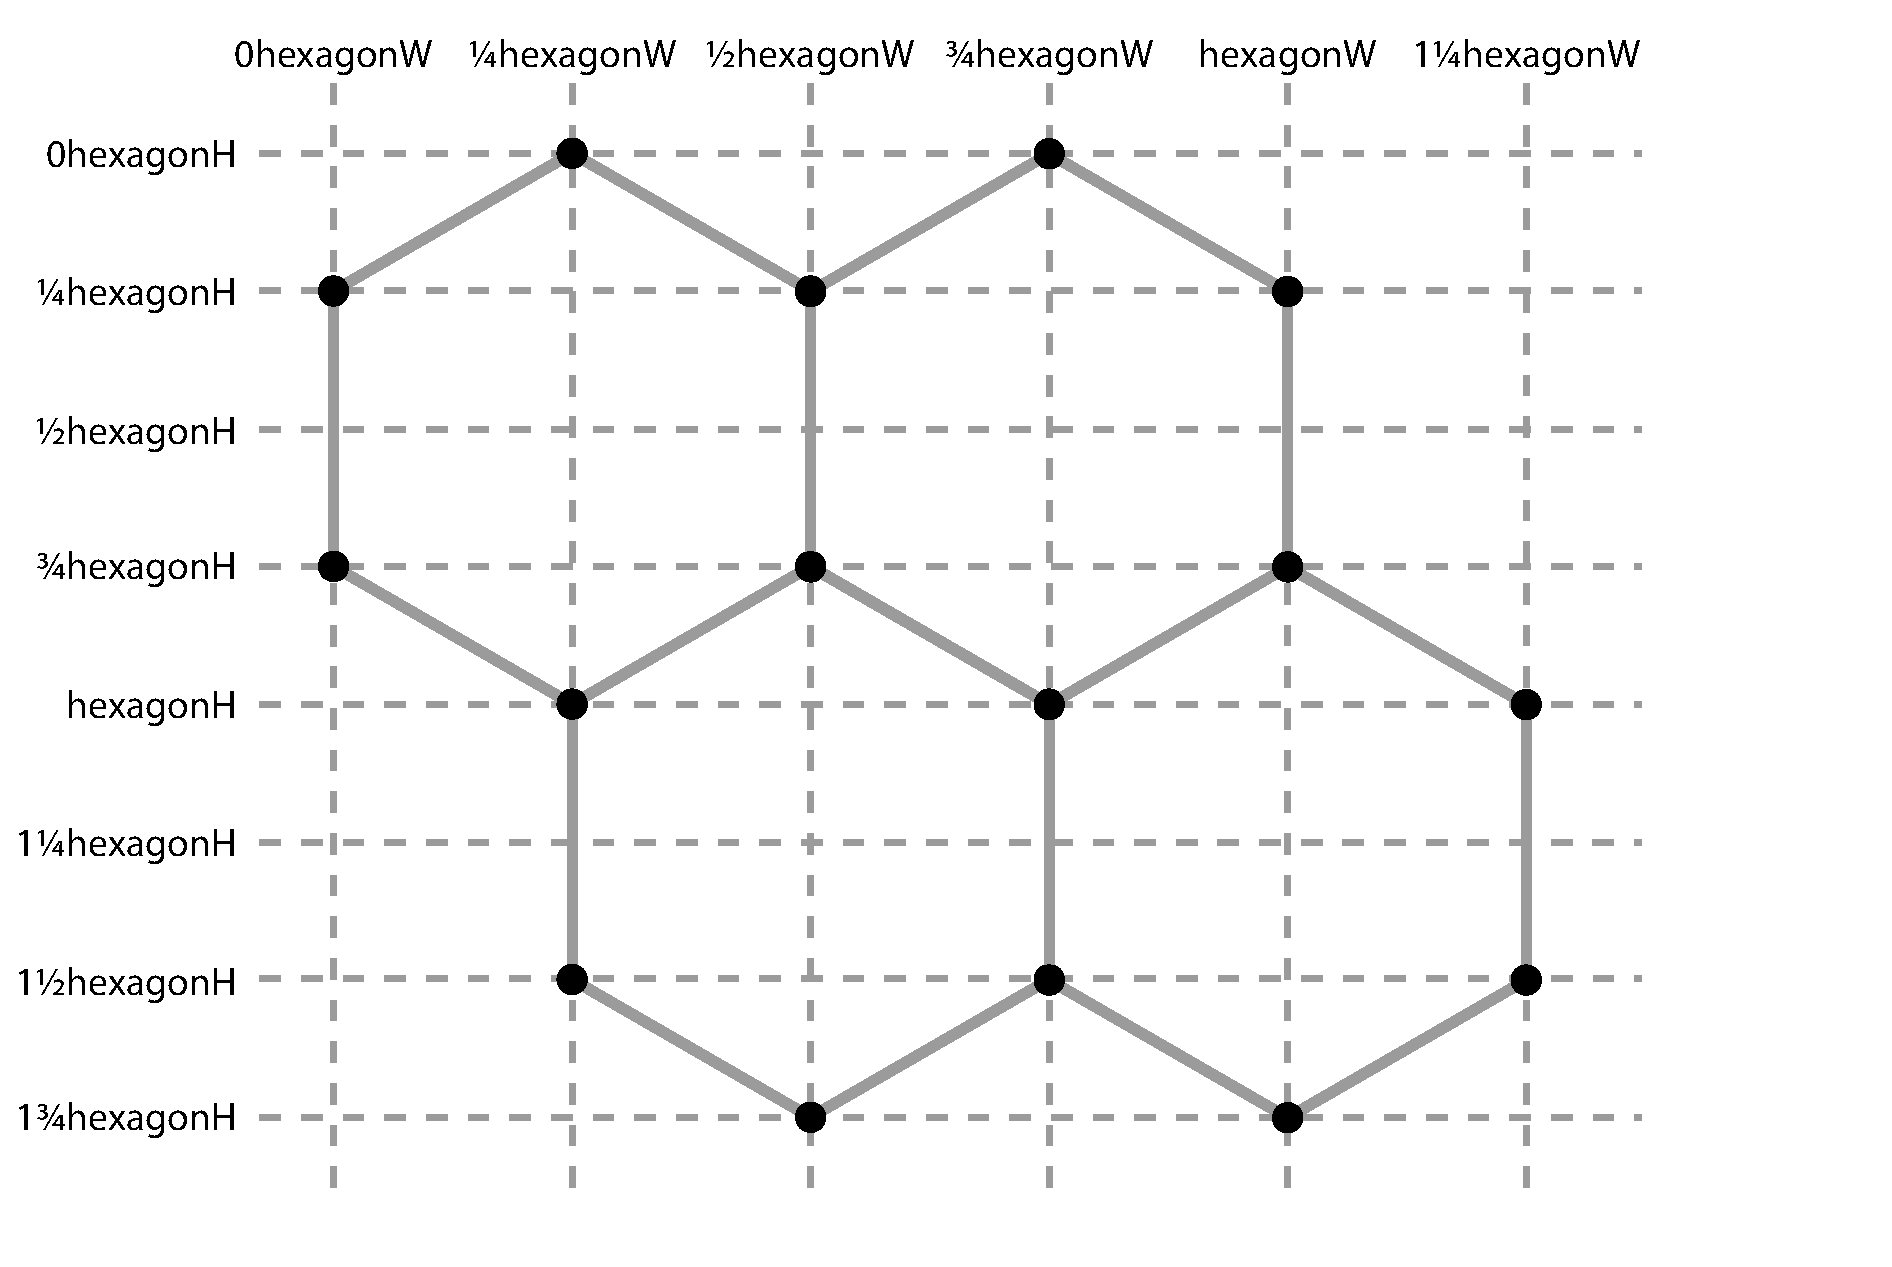
\includegraphics[height=0.35\textheight]{inc/img/hexagon_grid}
	\caption{Гексагональная сетка.}
	\label{analysis:hexagonGridWithPoints}
\end{figure}

Высота данного поля $gridHeight$ вычисляется по формуле: 
\begin{equation}
%\caption{Вычисление размера шестиугольника на основе ширины и высоты сетки.}
\label{hexGrid:gridHeight}
	gridHeight=hexH(\frac{3}{4}dimension+\frac{1}{4}),
\end{equation} 
где hexH --- высота шестиугольника, которую можно найти по формуле $2hexSize$. 
Ширина данного поля $gridWidth$ вычисляется по формуле: 
\begin{equation}
%\caption{Вычисление размера шестиугольника на основе ширины и высоты сетки.}
\label{hexGrid:gridWidth}
gridWidth=hexW\times dimension, 
\end{equation}
где hexW --- ширина 
шестиугольника, которая равна $hexSize\sqrt{3}$.

\section{Алгоритм Ли}
\label{analysis:li}

 \textbf{Алгоритм Ли} — волновой алгоритм поиска пути на карте, алгоритм трассировки. С его помощью можно построить путь, или трассу, между двумя любыми элементами в лабиринте. Из начального элемента распространяется в четырёх (в этой задаче — в 6) направлениях волна. Тот элемент, в который она пришла, образует фронт волны.

Элементы первого фронта волны являются источниками вторичных волн.

Элементы второго фронта генерируют волну третьего фронта и так далее. Процесс заканчивается тогда, когда достигается конечный элемент. На втором этапе строится трасса. Построение производится в соответствии с некоторыми правилами:
\begin{enumerate}
	\item при построении трассы движение проходит в зависимости от выбранных приоритетов,
	\item путевые координаты уменьшаются при переходе от начального элемента к конечному.
\end{enumerate}
Эти приоритеты выбираются в процессе разработки. В зависимости от выбора тех или иных приоритетов получаются различные трассы. Но в любом случае длина трассы остается одной и той же.

Используя волновой алгоритм, можно найти трассу в лабиринте с любым количеством стен. В этом и заключается \textbf{преимущество} его использования.

\textbf{Недостаток} алгоритма Ли заключается в том, что при построении трассы требуется большой объем памяти.







































%% !TEX root = 0-main.tex
% !TEX encoding = UTF-8 Unicode
\chapter{Проектирование программного инструмента}
\label{cha:ch_2}

Прежде всего выделим сущности и определим действия, которые необходимы для решения задачи.

\begin{enumerate}
\item \textbf{Правильный шестиугольник} характеризуется весом и координатой расположения на гексагональной сетке. В качестве допустимых действий можно выделить: изменение веса, сравнение с другими подобными сущностями.
\item \textbf{Гексагональная сетка} характеризуется размерностью. Определяет правила для создания, управления, хранения гексов. 
\end{enumerate}
Для формирования данных о гексагональной сетке рассмотрим варианты: загрузка данных из файла, редактирование (как новой, так и загруженной) гексагональной сетки в графическом режиме.

\section{Системы координат}
Для работы с элементами гексагональной сетки необходима система координат. Источник \cite{red} описывает три системы координат для прямоугольного дискретного 
рабочего поля (\textit{ПДРП}). Определим эти три системы для РТДРП и добавим еще одну: 

\subsection{Координаты смещений}
 Данная система определяет смещение шестиугольника в сетке относительно точки отсчета. Возьмем за точку отсчета верхний левый угол полотна, на котором будет отрисовываться сетка (Рис. \ref{axis:offset}).

\subsection{Порядковые координаты}
\label{design:ordinal_axis}
Первый показатель зависит от порядкового номера среди остальных элементов на одном уровне, относительно левого края. Второй соответсвует уровню, на котором элемент расположен (Рис. \ref{axis:ordinal}).\par
В ПДРП координаты смещений являются индексом элемента массива, 
который характеризует шестиугольник с данными координатами. Но в РТДРП вершина находится в середине рабочего поля. Так что порядковые координаты будут определять индекс с данными о шестиугольнике в соответствующей структуре хранения. 

\begin{figure}[h]
\begin{center}
\begin{minipage}[h]{0.47\linewidth}
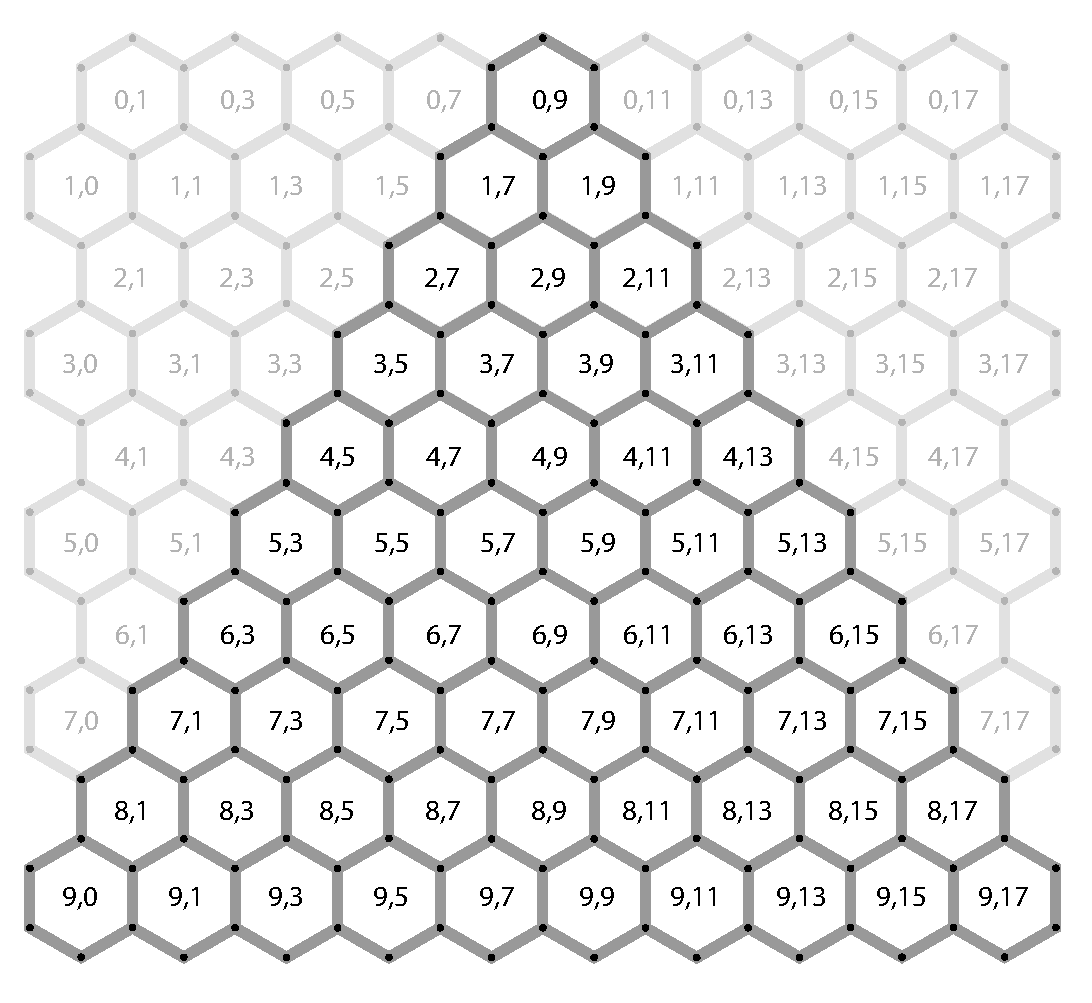
\includegraphics[width=1\linewidth]{inc/img/hexagon_offset}
\caption{Координаты смещений.} 
\label{axis:offset} 
\end{minipage}
\hfill 
\begin{minipage}[h]{0.47\linewidth}
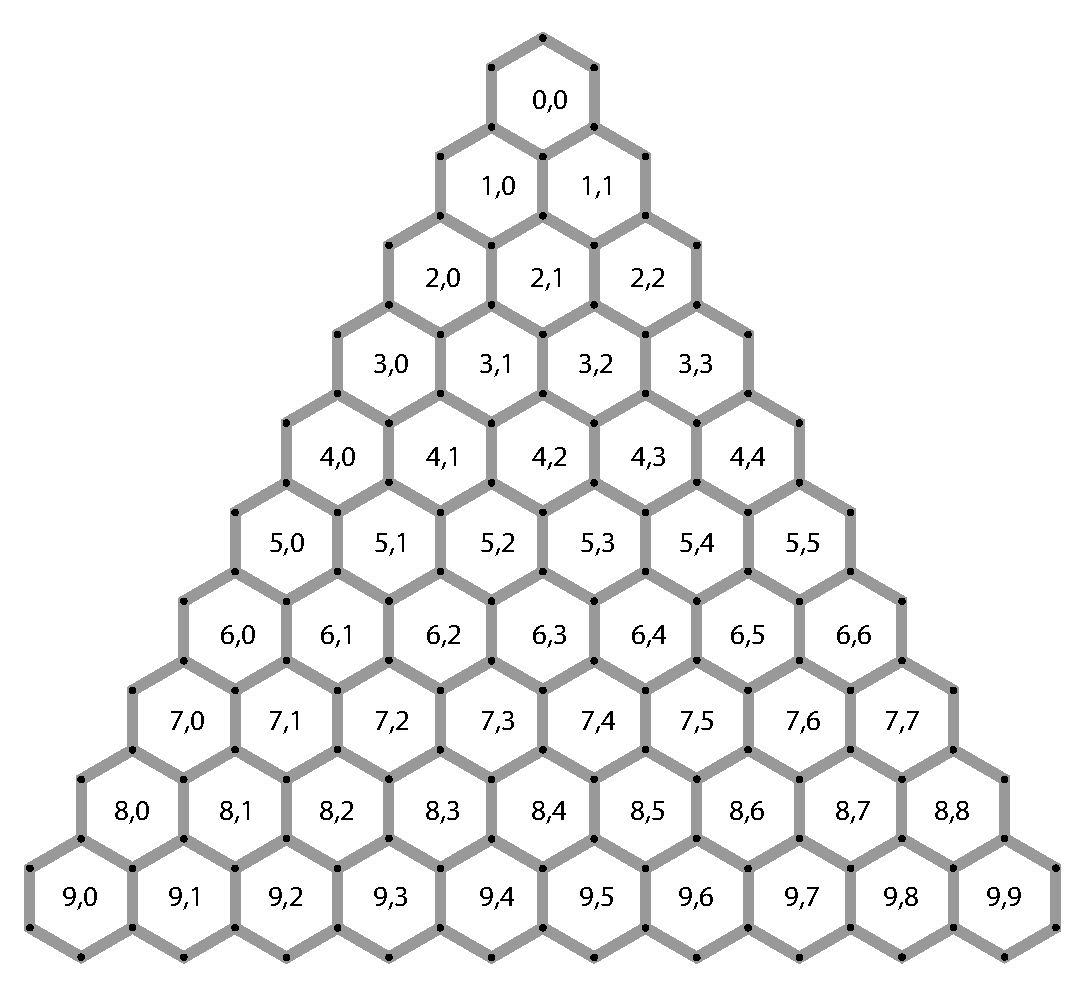
\includegraphics[width=1\linewidth]{inc/img/hexagon_ordinal}
\caption{Порядковые координаты.}
\label{axis:ordinal}
\end{minipage}
\end{center}
\end{figure}

\subsection{Кубические координаты}
Данная система имеет три оси координат \textit{X, Y, Z}. Согласно \cite{red}, берется сетка кубов в этой системе координат и из нее вырезается диагональная плоскость $x+y+z=0$. (Рис. \ref{axis:cube})

\par
Для вычисления центра системы координат относительно порядковой координаты, необходимо найти точку пересечения биссектрис равностороннего треугольника,  в который помещается гексагональная сетка.
$centerHexagon_{y} = 2\lfloor gridD / 3\rfloor $ --- ряд гексагональной сетки, где координата по оси $Z$ равна $0$.
$centerHexagon_{x} = centerR / 2 $ --- позиция шестиугольника в ряду $centerR$, у которого все координаты $0$.
\par Данная система удобна для различных арифметических действий с координатами элементов (можно воспользоваться стандартными операциями из декартовых координат: суммированием и вычитанием координат, умножением и делением на скалярную величину, а также расстояниями) и отлично подходит для работы с алгоритмами на графах.

\subsection{Осевые координаты}
Осевая система координат, иногда называемая «трапецеидальной», строится на основе двух или трёх координат из кубической системы координат. Поскольку у нас есть условие x + y + z = 0, третья координата не нужна. Осевые координаты полезны для хранения карт и отображения координат пользователю. Как и в случае с кубическими координатами, с ними можно использовать стандартные операции суммирования, вычитания, умножения и деления декартовых координат.\par
Преимущество этой системы перед сетками смещений в большей понятности алгоритмов. Недостатком системы является то, что хранение прямоугольной карты выполняется нелинейным способом. Некоторые алгоритмы ещё понятнее в кубических координатах, но поскольку есть условие $x + y + z = 0$, значит  можно вычислить третью подразумеваемую координату и использовать её в этих алгоритмах (Рис. \ref{axis:axial}).

\begin{figure}[h]
\begin{center}
\begin{minipage}[h]{0.47\linewidth}
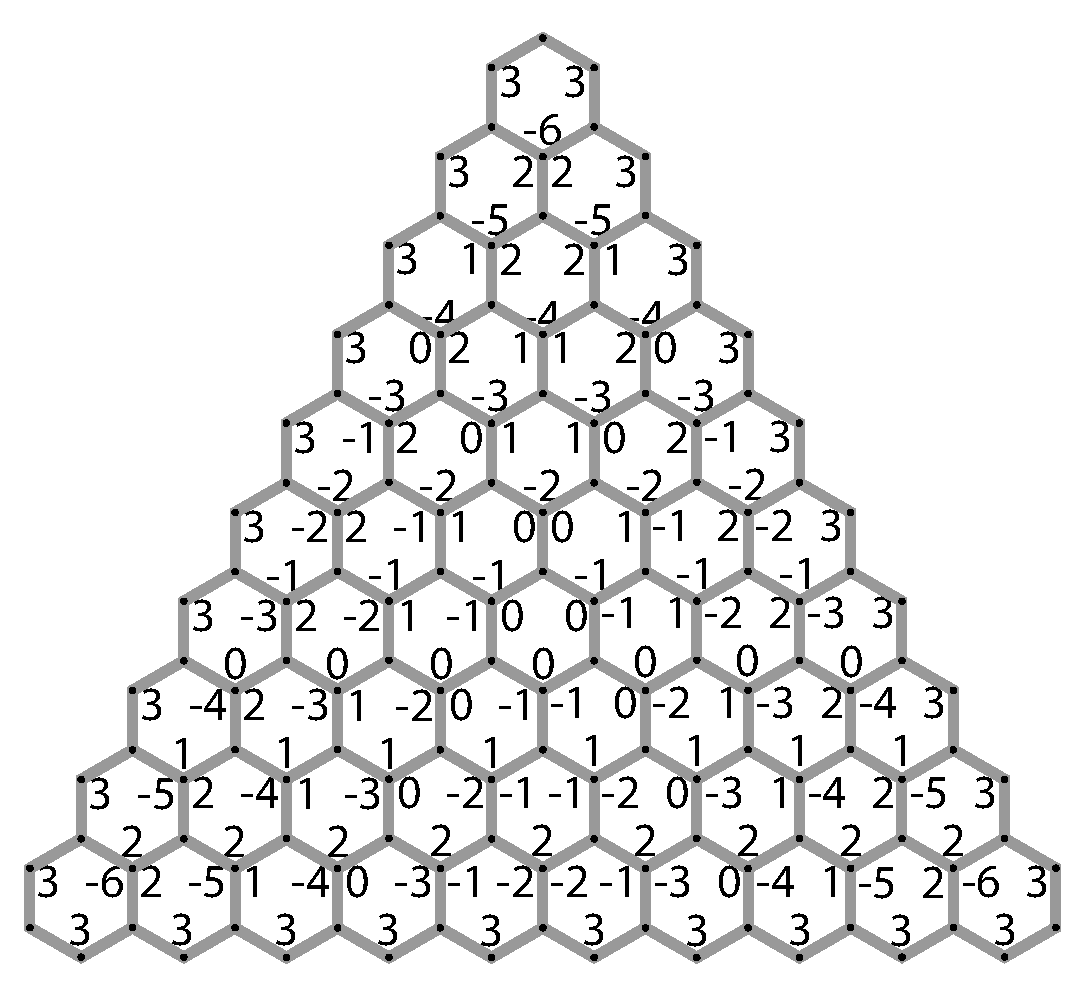
\includegraphics[width=1\linewidth]{inc/img/hexagon_cube}
\caption{Кубические координаты.} %% подпись к рисунку
\label{axis:cube} %% метка рисунка для ссылки на него
\end{minipage}
\hfill 
\begin{minipage}[h]{0.47\linewidth}
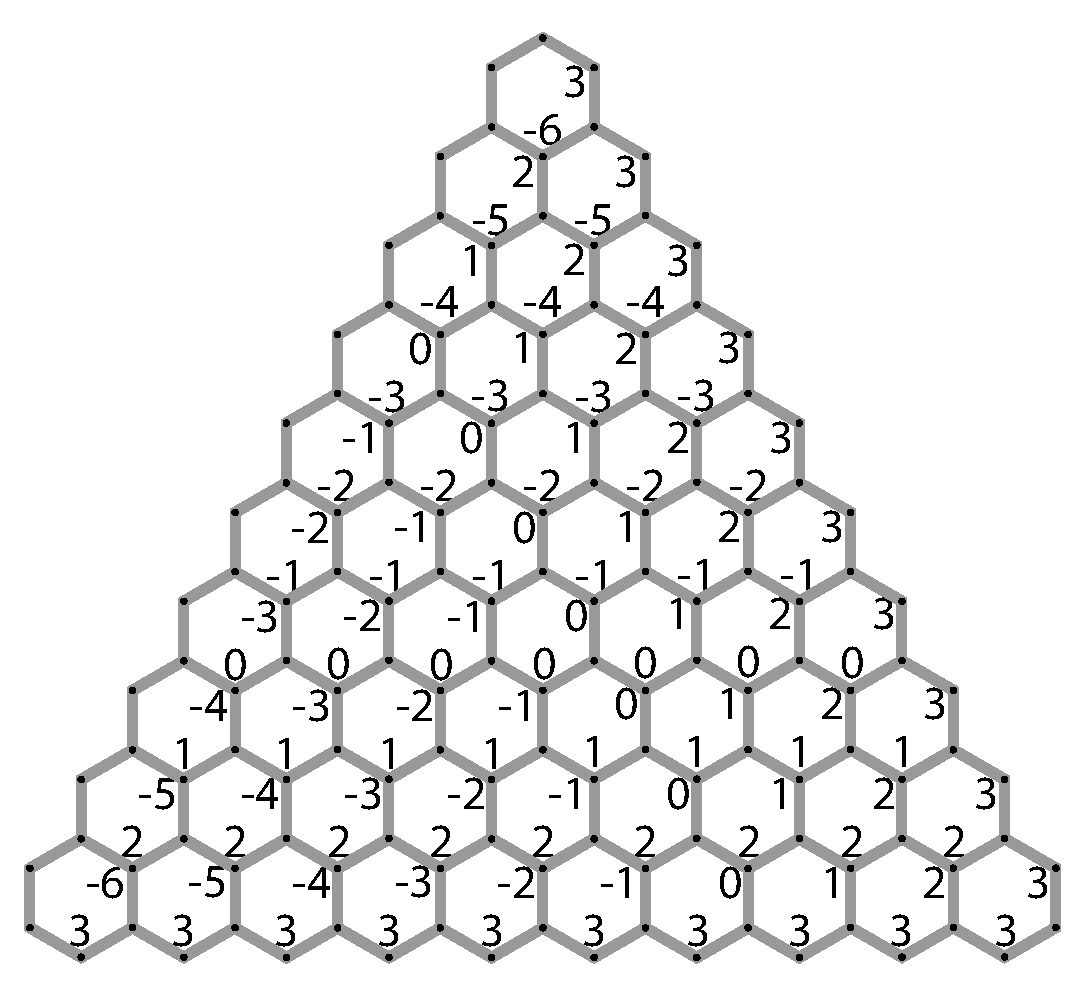
\includegraphics[width=1\linewidth]{inc/img/hexagon_axial}
\caption{Осевые координаты.}
\label{axis:axial}
\end{minipage}
\end{center}
\end{figure}

\section{Проектирование реализации алгоритма Дейкстры}
Данный алгоритм, согласно теории (раздел \ref{analysis:dijkstra}), работает со взвешенным орграфом. Пусть вершина --- это шестиугольник в орграфе, а вес дуги задается весом конечной вершины, так как это является водным условием задачи (Рис.\ref{hexagon:weight}).
\begin{figure}[h]
	\centering
	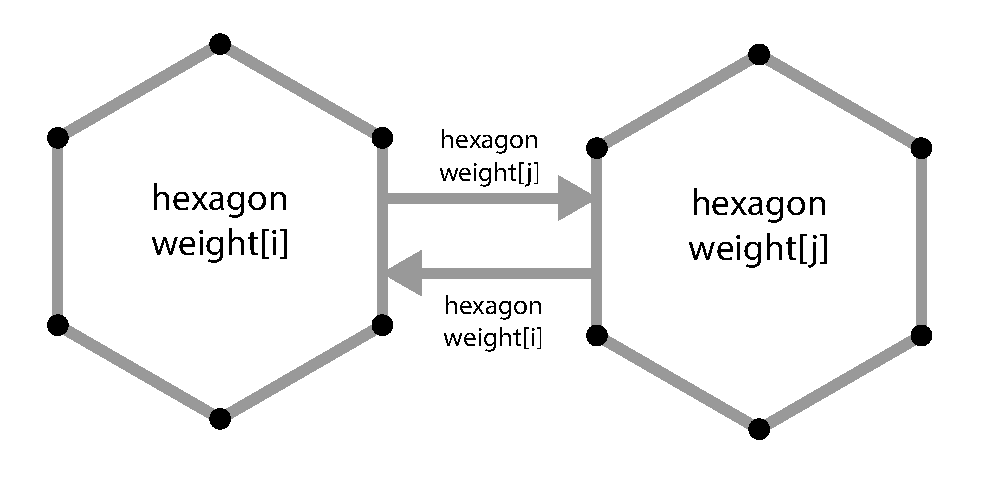
\includegraphics[height=0.3\textwidth]{inc/img/hexagon_weight}
	\caption{Определение веса шестиугольника.}
	\label{hexagon:weight}
\end{figure}
\par
Тогда, входными данными алгоритма является гексагональная сетка, начало и конец искомого пути.
\par Для упрощения структуры хранения гексагональной сетки можно ввести функцию нахождения соседних шестиугольников на основе кубических координат. Для этого необходимо вектор координат шестиугольника сложить поочередно с каждым из шести векторов $
\Bigg( 
\begin{bmatrix}-1\\1\\0\end{bmatrix},
\begin{bmatrix}1\\-1\\0\end{bmatrix},
\begin{bmatrix}0\\-1\\1\end{bmatrix},
\begin{bmatrix}0\\1\\-1\end{bmatrix},
\begin{bmatrix}1\\0\\-1\end{bmatrix}, 
\begin{bmatrix}-1\\0\\1\end{bmatrix}
\Bigg)
$вычисления соседа (Рис. \ref{hexagon:neighbors}), не забывая, что у элементов на границе РТДРП их количество равно или 4, или 2 (на вершинах РТДРП).   
\begin{figure}[h]
	\centering
	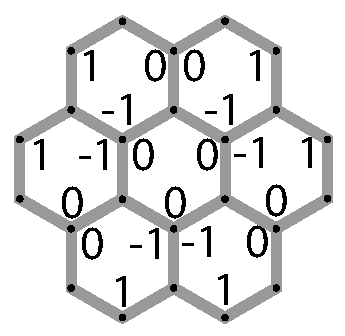
\includegraphics[height=0.3\textwidth]{inc/img/neib}
	\caption{Координаты для вычисления соседних шестиугольников.}
	\label{hexagon:neighbors}
\end{figure}
\par

\section{Проектирование графического интерфейса}
Консольное приложение реализуется в разы быстрее, чем с графическим интерфейсом. Относительно данной задачи неудобство консольного связано с вводом и выводом данных. При размерности РТДРП равной 100 будет необходимо ввести 5050 параметров каждого шестиугольника. А при правильном подходе к тестированию, возникнет необходимость в создании специализированных входных данных, которые позволят отследить работоспособность и правильность работы алгоритма. Редактирование такого количества данных потребует времени. А графический интерфейс позволит редактировать данные прямо на графическом представлении гексагональной сетки, что в разы сэкономит время и силы. Так же появляется возможность наглядно отслеживать работу алгоритма.
\par
Для этого необходимо разработать:
\begin{enumerate}
	\item Дизайн и логику главного окна;
	\item Отрисовку гексагональной сетки;
	\item Возможность взаимодействия с гексагональной сетки с помощью компьютерной мыши;
	\item Наглядное представление работы алгоритма Дейкстры.
\end{enumerate}
\subsection{Главное окно}
Необходимо предоставить возможность пользователю с помощью графического интерфейса создавать, открывать, редактировать и сохранять гексагональные сетки. А также воспроизводить алгоритм Дейкстры, отображать и сохранять его результат и промежуточные данные работы. Для этих задач необходимо в главном окне разместить соответсвующие кнопки для управления согласно ситуации. 
\subsection{Отрисовка гексагональной сетки}
\label{design:paint_hex_grid}
После запуска программы и инициирования создания новой или открытия сохраненной гексагональной сетки необходимо определиться с её размерами, чтобы РТДРП полностью помещалась в соотвествующий раздел главного окна. Согласно формулам \ref{hexGrid:gridHeight} и \ref{hexGrid:gridWidth} можно вычислить размер шестиугольника, взяв за $gridH$ высоту раздела или $gridW$ ширину раздела. Но для того, чтобы сетка точно поместилось, необходимо определить $min(gridH, gridW)$ и по соответствующей далее формуле (\ref{hexagon:sizeByGridHeight} или \ref{hexagon:sizeByGridWidth})  вычислить $hexagonSize$.
\begin{equation}
%\caption{Вычисление размера шестиугольника на основе ширины и высоты сетки.}
\label{hexagon:sizeByGridHeight}
hexagonSize = \frac{gridH}{2( \frac{3}{4}gridD+\frac{1}{4} )}
\end{equation}

\begin{equation}
%\caption{Вычисление размера шестиугольника на основе ширины и высоты сетки.}
\label{hexagon:sizeByGridWidth}
hexagonSize = \frac{gridW\sqrt{3}}{3\times gridD}
\end{equation}
Все необходимые данные для отрисовки гескагональной сетки собраны. Теперь необходимо описать шестиугольник, для его отрисовки. Согласно рисунку \ref{analysis:hexagonGridWithPoints}, зададим формулы для вычисления координаты в системе, где будет отображаться сетка. 
\par 
Из теории о координатах заметим, что на каждом ряду (уровне) сетки крайний левый шестиугольник начинает свое <<движение>> с середины (шестиугольник $(0,0)$ на Рис. \ref{axis:ordinal}) и до левой границы РТДРП (шестиугольник $(9,0)$ на Рис. \ref{axis:ordinal}). Воспользуемся данным замечанием и выведем формулу для этого элемента $leftHexagon_{level_{x}}$, это позволит воспользоваться логикой порядковых координат (раздел \ref{design:ordinal_axis}) и вычислять последующие элементы данного уровня.
\begin{equation}
%\caption{Вычисление размера шестиугольника на основе ширины и высоты сетки.}
\label{hex:leftHex}
leftHexagon_{level_{x}} = centerHexagon_{x} - \frac{r}{2}hexagonWidth
\end{equation}
Согласно вышеупомянутой теории и формулам, вычислим координаты точек, образующих шестиугольник.
\begin{figure}[h]
	\centering
	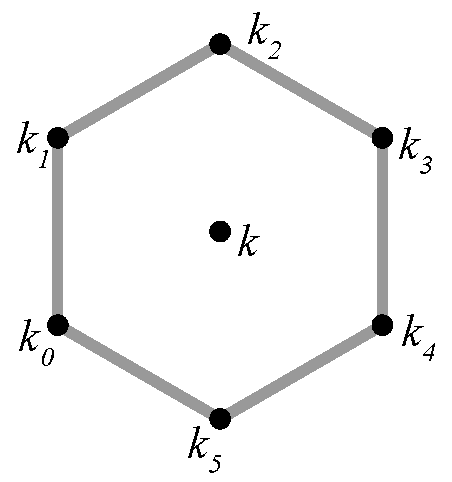
\includegraphics[width=0.25\linewidth]{inc/img/hexagon_edges}
	\caption{}
	\label{fig:}
\end{figure}


\begin{equation}
\begin{aligned}
&k \{leftHexagon_{level_{x}} + hexagonWidth\times currentHexagon_{level};  \\
&\hspace{3mm}\frac{1}{2} hexagonHeight +\frac{3}{4} hexagonHeight\times currentHexagon_{ordinal_{x}}\},  \\
&k_{0}\{k_{x}-\frac{1}{2}hexagonWidth; k_{y}+\frac{1}{4}hexagonHeight\},  \\
&k_{1}\{k_{x}-\frac{1}{2}hexagonWidth; k_{y}-\frac{1}{4}hexagonHeight\},  \\
&k_{2}\{k_{x};k_{y}-\frac{1}{2}hexagonHeight\},  \\
&k_{3}\{k_{x}+\frac{1}{2}hexagonWidth; k_{y}-\frac{1}{4}hexagonHeight\},  \\
&k_{4}\{k_{x}+\frac{1}{2}hexagonWidth; k_{y}+\frac{1}{4}hexagonHeight\},  \\
&k_{5}\{k_{x};k_{y}+\frac{1}{2}hexagonHeight\}.
\end{aligned}
%\phantom{\hspace{6cm}} %%<---adjust the value as you want
\end{equation}
Осталось назначить цвет каждому шестиугольнику. Весьма логично связать гексагональную сетку с <<трудно проходимым лесом>>, в котором вес шестиугольника --- <<стоимость>> или <<сложность>> прохождения данного участка.

\begin{figure}[h]
\begin{center}
\begin{minipage}[h]{0.47\linewidth}
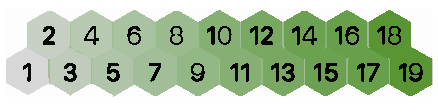
\includegraphics[width=1\linewidth]{inc/img/hexagon_gradient}
\caption{Пример раскраски гексагональной сетки.} %% подпись к рисунку
\label{axis:cube} %% метка рисунка для ссылки на него
\end{minipage}
\hfill 
\begin{minipage}[h]{0.47\linewidth}
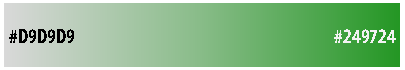
\includegraphics[width=1\linewidth]{inc/img/gradient}
\caption{Цветовой градиент раскраски шестиугольника.}
\label{axis:axial}
\end{minipage}
\end{center}
\end{figure}

Для \textbf{создания svg файла} будут использоваться аналогичные методики и формулы.
\subsection{Взаимодействия с гексагональной сетки}

Взаимодействие будет происходить с помощью компьютерной мыши. Можно выделить несколько способов определения нужного шестиугольника и один из самых простых --- это перебор и сравнение координат нажатия относительно координат вершин шестиугольников, но это нерационально, особенно при больших размерах. Другой --- конвертировать координату нажатия относительно осевых координат. Для этого необходимо:
\begin{enumerate}
	\item Сместить систему координат мыши относительно центра осевой системы координат. В результате, координаты нажатия изменятся относительно смещения;
	\item Далее, необходимо сделать поворот осей мыши на 60\degree. То есть, вектор координат умножаем на матрицу поворота $\begin{bmatrix}\sqrt{3}/3& -1/3\\0& 2/3\end{bmatrix}$;
	\item В заключении, осуществим целочисленное деление (без округления) координат на $2\times hexagonSize$. 
\end{enumerate}
%TODO Вставить изображения
\begin{figure}[h]
\begin{center}
\begin{minipage}[h]{0.47\linewidth}
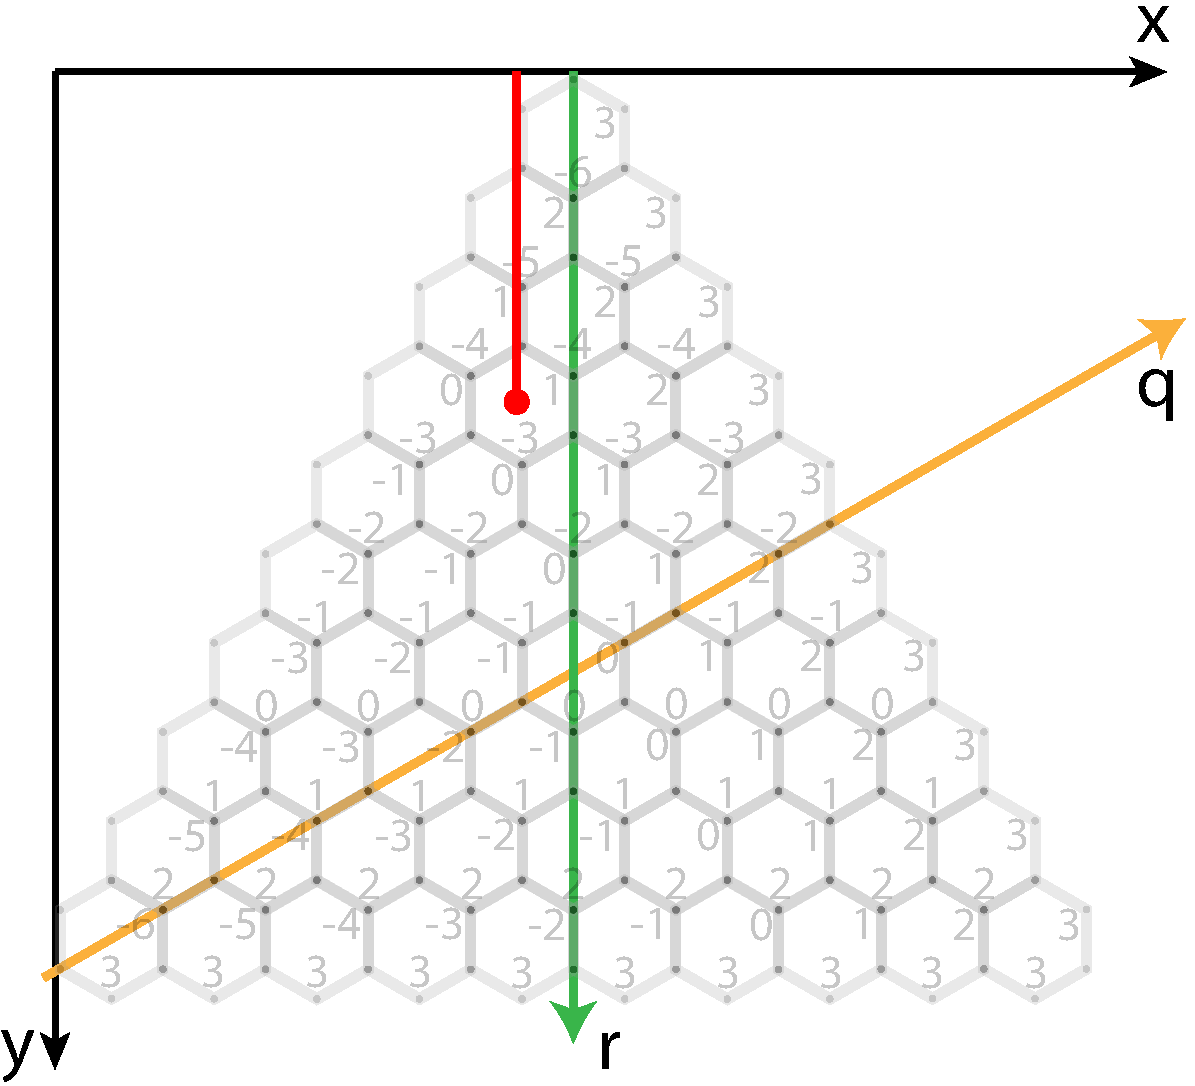
\includegraphics[width=1\linewidth]{inc/img/calcPoint_two}
\caption{Проекция координаты нажатия на ось $X$.} %% подпись к рисунку
\label{axis:cube} %% метка рисунка для ссылки на него
\end{minipage}
\hfill 
\begin{minipage}[h]{0.47\linewidth}
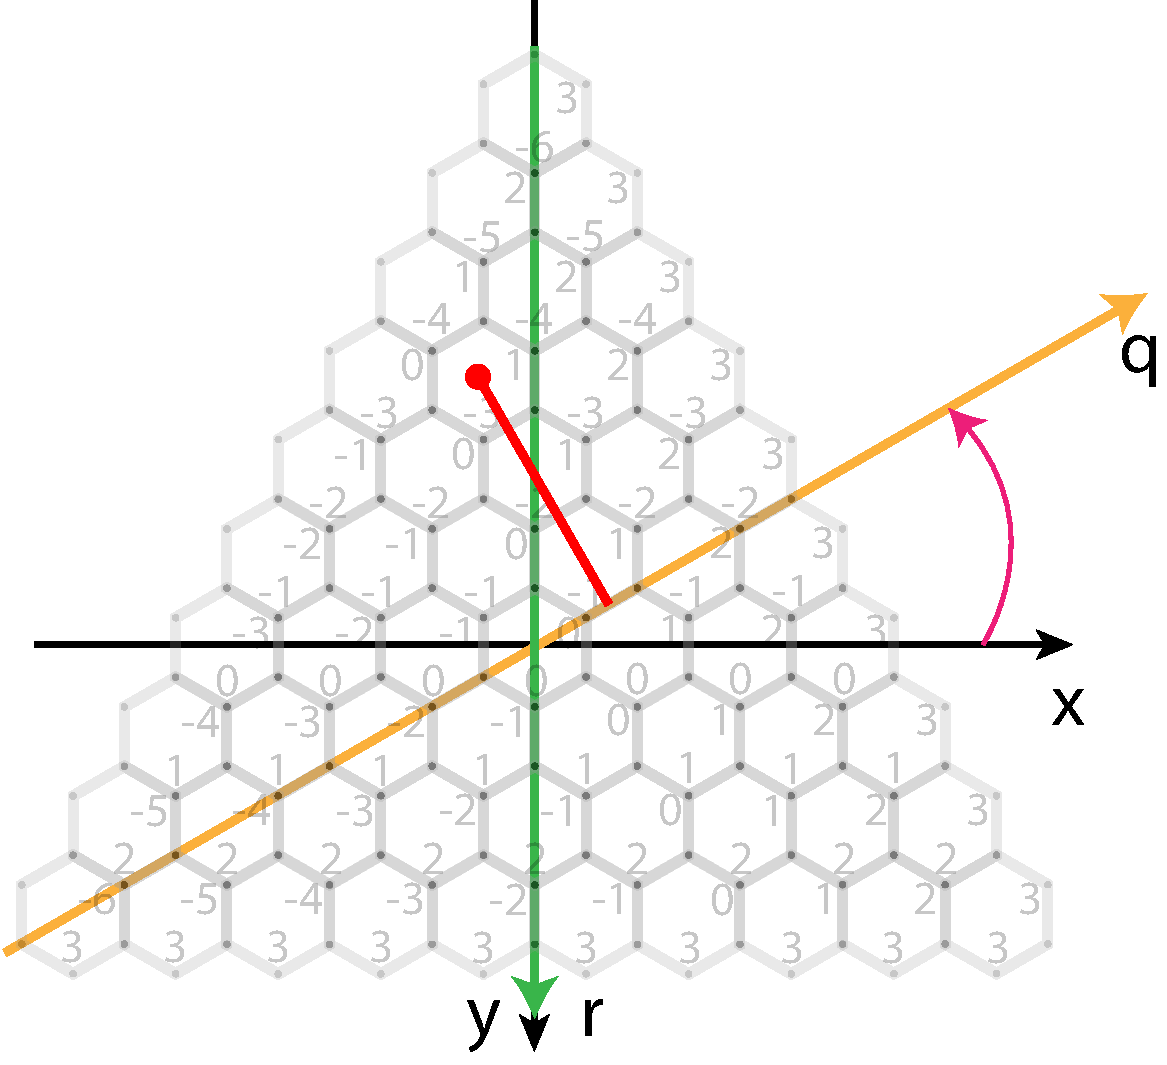
\includegraphics[width=1\linewidth]{inc/img/calcPoint_three}
\caption{Проекция координаты нажатия на ось $Q$.}
\label{axis:axial}
\end{minipage}
\end{center}
\end{figure}

\subsection{Проектирование вывода результата работы алгоритма Дейкстры}
Согласно теории (раздел \ref{analysis:dijkstra}), результатом работы алгоритма является вектор с длинами кратчайших путей из начала до всех остальных вершин. Следовательно, в качестве результата и промежуточного результата работы алгоритма целесообразно брать этот вектор и в качестве веса шестиугольника отображать длину (стоимость, сложность) кратчайшего пути до него.
%% !TEX root = 0-main.tex
% !TEX encoding = UTF-8 Unicode

\chapter{Реализация программного инструмента}
\label{cha:ch_3}
Архитектура программного инструмента построена согласно парадигме объектно-ориентированного программирования. В качестве условий разделения данных в приложении использовался метод <<Модель-Представление-Контроллер>>(MVC).

\begin{longtable}[c]{|p{2cm}|p{2cm}|p{2cm}|p{8cm}|}
\hline
\multicolumn{1}{|p{2cm}|}{\textbf{Тип возвращаемого элемента}} & \multicolumn{1}{p{2cm}|}{\textbf{Имя}} & \multicolumn{1}{p{2cm}|}{\textbf{Параме\-тры}} & \multicolumn{1}{c|}{\textbf{Назначение}}                                                                     \\ \hline
\endfirsthead
%
\endhead
%
void                                                      & HexGrid\-Layout                     & QWidget *parent = nullptr               & Конструктор виджета, описывающего работу виджета гексагональной сетки и управляющих элементов (кнопок, меню) \\ \hline
void                                                      & openFile                          &                                         & Позволяет пользователю выбрать файл для чтения в ситле ОС                                                    \\ \hline
void                                                      & saveHex\-Grid                       &                                         & Позволяет пользователю выбрать место для сохранения и имя файла с данными о гексагональной сетке             \\ \hline
void                                                      & create\-NewHex\-Grid                  & int lenght=0                            & Создает новую гексагональную сетку (отображение и модель)                                                    \\ \hline
void                                                      & closeCur\-rentHex\-Grid               &                                         & Удаляет отображение и модель актуальной гексагональной сетки                                                 \\ \hline
void                                                      & saveAllIt\-erations&                                         & Позволяет пользователю выбрать папку для для сохранения всех итераций работы алгоритма в формате SVG         \\ \hline
void                                                      & doDijks\-tra                        & bool bySteps = false                    & Выполняет алгоритм на актуальной сетке с возможностью поэтапного выполнения                                  \\ \hline
\caption{Методы класса HexGridLayout с модификатором доступа public}
\label{my-label}\\
\end{longtable}


\begin{longtable}[c]{|p{2cm}|p{2cm}|p{2.3cm}|p{7.7cm}|}
\\
\hline
\multicolumn{1}{|p{2cm}|}{\textbf{Имя}} & \multicolumn{1}{p{2cm}|}{\textbf{Мод. доступа}} & \multicolumn{1}{p{2cm}|}{\textbf{Параме\-тры}}                      & \multicolumn{1}{p{8cm}|}{\textbf{Назначение}}                                                                                                      \\ \hline
\endfirsthead
%
\endhead
%
HexGrid\-View                       & public                                     & Triangular\-HexGraph **hexGrid\-Model, QWidget *parent = nullptr & Конструктор виджета для отображения гексагональной стеки. В качестве параметра передается указатель на указатель модели гексагональной стеки. \\ \hline
openMou\-seSetti\-ngsWidget           & public                                     &                                                              & Отображается диалоговое окно с настройками управления гексагональной сетки                                                                    \\ \hline
choose\-Start\-Hex                    & public                                     &                                                              & После вызова позволяет выбрать стартовый шестиугольник                                                                                        \\ \hline
choose\-Finish\-Hex                   & public                                     &                                                              & После вызова позволяет выбрать финишный шестиугольник                                                                                         \\ \hline
paint\-Event                        & protected                                  & QPaint\-Event*                                                 & Метод, который отрисовывает шестиугольную сетку                                                                                               \\ \hline
mouse\-Press\-Event                   & private                                    & QMouse\-Event*~pe                                              & Метод, который обрабатывает нажатие кнопки мыши       
\\ \hline  
\caption{Методы класса TriangularHexGrap с возвращаемым типом данных void.}
\label{my-label}\\                                                                                     
\end{longtable}

% Please add the following required packages to your document preamble:
% \usepackage{longtable}
% Note: It may be necessary to compile the document several times to get a multi-page table to line up properly
\begin{longtable}[c]{|p{2.2cm}|p{2.1cm}|p{2.2cm}|p{7.6cm}|}
\hline
\multicolumn{1}{|p{2cm}|}{\textbf{Тип возвращаемого элемента}} & \multicolumn{1}{p{2cm}|}{\textbf{Имя}} & \multicolumn{1}{p{2cm}|}{\textbf{Параме\-тры}} & \multicolumn{1}{c|}{\textbf{Назначение}}                                                                     \\ \hline
\endfirsthead
%
\endhead
%
void                                                      & Trian\-gular\-Hex\-Graph                & unsigned lenght                                                                                                                       & Конструктор класса, передается размерность гексагональной сетки                          \\ \hline
void                                                      & setHex\-Size                        & double hexSize                                                                                                                        & Задаем размер шестиугольника, на основе которых вычисляются другие характеристики сетки  \\ \hline
HexCube                                                   & toCube\-fromOffset                  & HexCoord row, HexCoord column                                                                                                         & Конвертирует из порядковых координат в кубические                                        \\ \hline
                                                          & toCube\-FromAxial                   & HexCoord q, HexCoord r                                                                                                                & Конвертирует из осевых координат в кубические                                            \\ \hline
HexData                                                   & getWeight                         & HexCube cube                                                                                                                          & Возвращает вес шестиугольника по кубическим координатам                                  \\ \hline
Void                                                      & setPlus\-Weight                     & HexData increment, HexCoord row, HexCoord column                                                                                      & Увеличивает вес шестиугольника на increment                                              \\ \hline
                                                          & setMinus\-Weight                    & HexData decrement, HexCoord row, HexCoord column                                                                                      & Уменьшает вес шестиугольника на decrement, с учетом того, что вес не может быть меньше 1 \\ \hline
std::vector\-\textless{}svg::\-Point\textgreater{}            & getHex\-Edge\-Points                  & HexCoord row, HexCoord column                                                                                                         & Возвращает вектор с координатами вершин шестиугольника для отрисовки                     \\ \hline
std::vector\-\textless{}Hex\textgreater{}                   & neighbors                         & HexCoord row, HexCoord column                                                                                                         & Возвращает  вектор с координатами соседей шестиугольника                                 \\ \hline
Void                                                      & drawSVG\-with\-Frontier               & std::map\-\textless{}Hex\-Cube, Hex\-Data\textgreater{}* frontiers, std::vector\-\textless{}Hex\-Cube\textgreater{}* path, std::string fileName & Создает SVG файл с гексагональной сеткой и фронтами алгоритма                            \\ \hline
\caption{Методы класса TriangularHexGrap с модификатором доступа public.}
\label{my-label}\\
\end{longtable}
%\chapter{Описание работы программы}
\label{cha:ch_4}


Программа представляет собой исполняемый пакет (для Unix подобных операционных систем), для ее работы не требуется наличие специализированных программ и библиотек.
\par

После запуска программы пользователю предоставляется выбор: создать новую гексагональную сетку или загрузить. При создании новой сетки, появится диалоговое окно, в котором необходимо задать размерность РТДРП. После этого в главном окне появится графическое представление сетки, которое можно редактировать с помощью нажатия левой клавиши мыши (ЛКМ) для увеличение веса выбранного шестиугольника, или правой клавишей мыши (ПКМ) --- для уменьшение. Есть возможность редактирования сетки при зажатой ЛКМ и ПКМ.
\par

\begin{figure}[h]
\begin{center}
\begin{minipage}[h]{0.47\linewidth}
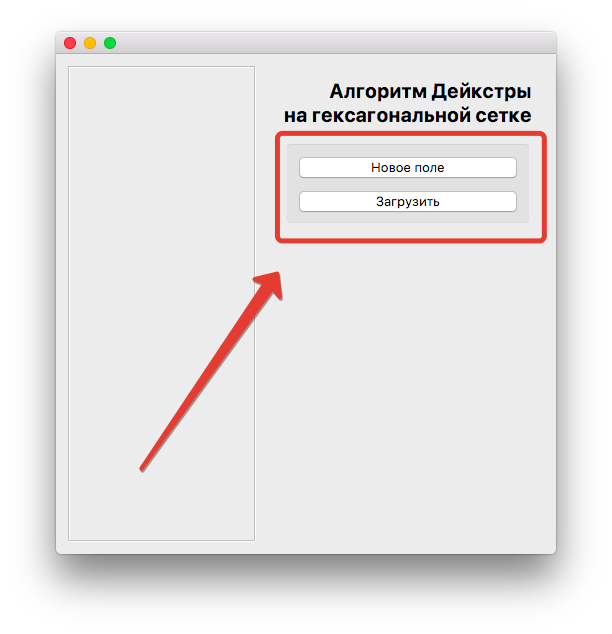
\includegraphics[width=1\linewidth]{inc/img/menuWitCreate}
\caption{Правое боковое меню при отсутствии сетки.} %% подпись к рисунку
\label{axis:cube} %% метка рисунка для ссылки на него
\end{minipage}
\hfill 
\begin{minipage}[h]{0.47\linewidth}
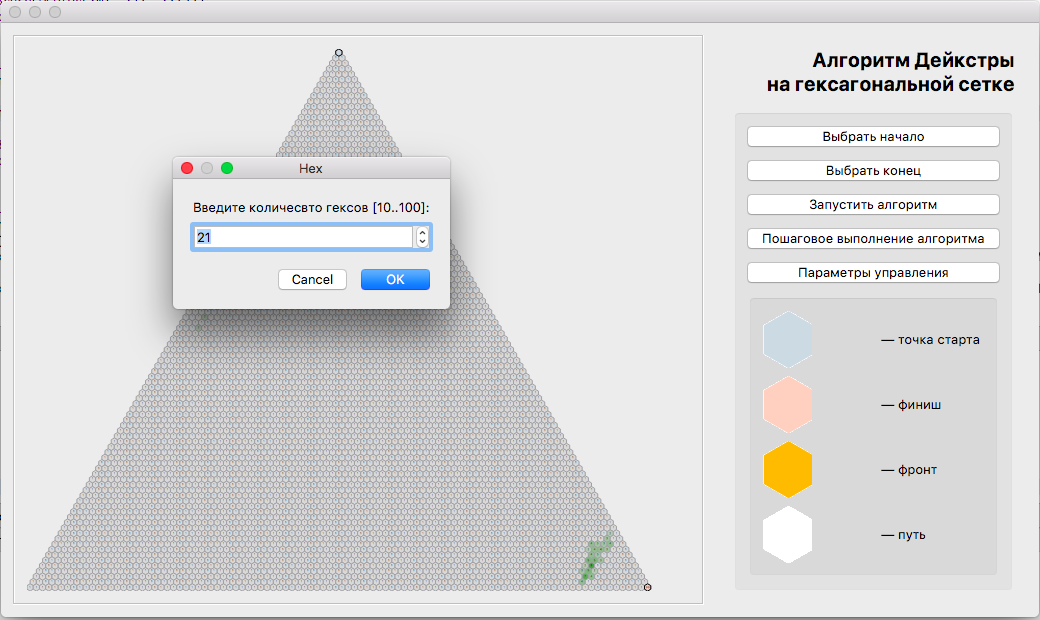
\includegraphics[width=1\linewidth]{inc/img/numOfElems}
\caption{Диалоговое окно, для ввода количества элементов РТДРП.}
\label{axis:axial}
\end{minipage}
\end{center}
\end{figure}

\begin{figure}[h]
\begin{center}
\begin{minipage}[h]{0.47\linewidth}
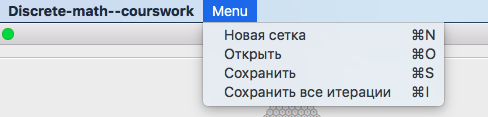
\includegraphics[width=1\linewidth]{inc/img/menu}
\caption{Меню программы.} %% подпись к рисунку
\label{axis:cube} %% метка рисунка для ссылки на него
\end{minipage}
\hfill 
\begin{minipage}[h]{0.47\linewidth}
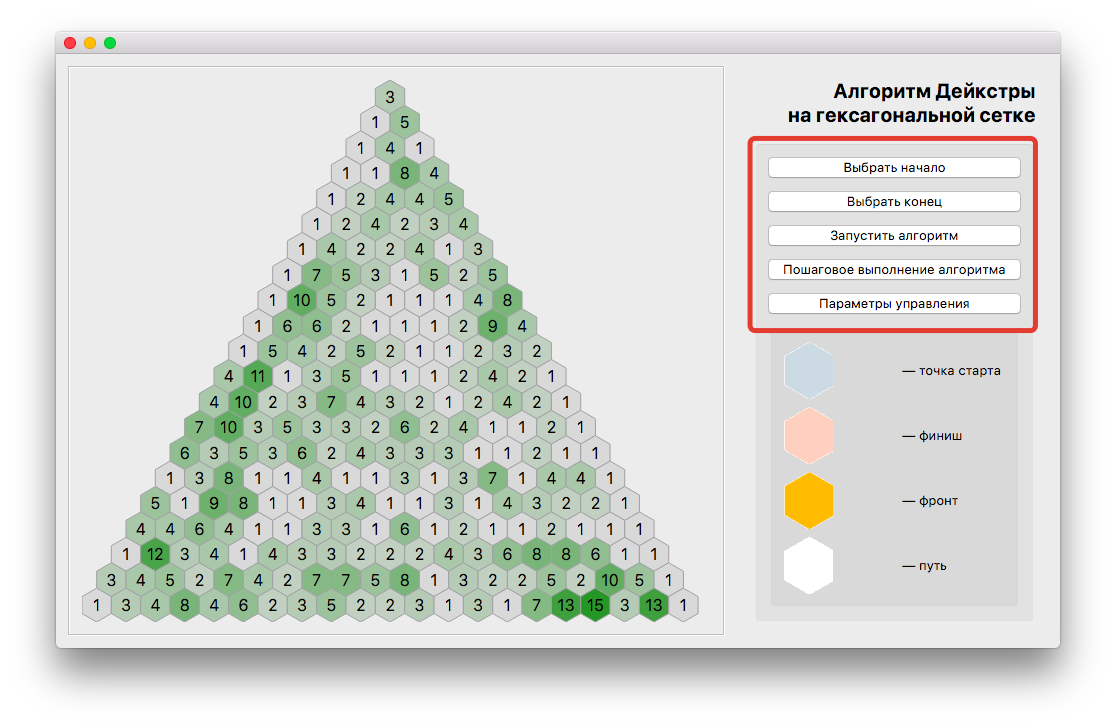
\includegraphics[width=1\linewidth]{inc/img/doSomeThings}
\caption{Правое боковое меню, для выбора действий над сеткой.}
\label{axis:axial}
\end{minipage}
\end{center}
\end{figure}

Перед запуском алгоритма Дейкстры необходимо выбрать начало и конец пути. Для этого в правом боковом меню главного окна необходимо выбрать <<Выбрать начало>>, далее, нажать на желаемый шестиугольник, выбрать в боковом меню <<Выбрать конец>> и нажать на соотвествующий элемент гексагональной сетки. После этого \textbf{возможно} выполнение алгоритма. Для этого необходимо нажать на кнопку в боковом меню <<Запустить алгоритм>>, в результате чего результат сразу отобразится на графическом представлении, или можно выполнить алгоритм пошагово. После каждого нажатия на <<Пошаговое выполнение алгоритма>> на графическое представление будут добавляться шестиугольники, которые добавлены в вектор с длинами кратчайших путей из начала до пройденным элементам. \par

\begin{figure}[h]
\begin{center}
\begin{minipage}[h]{0.47\linewidth}
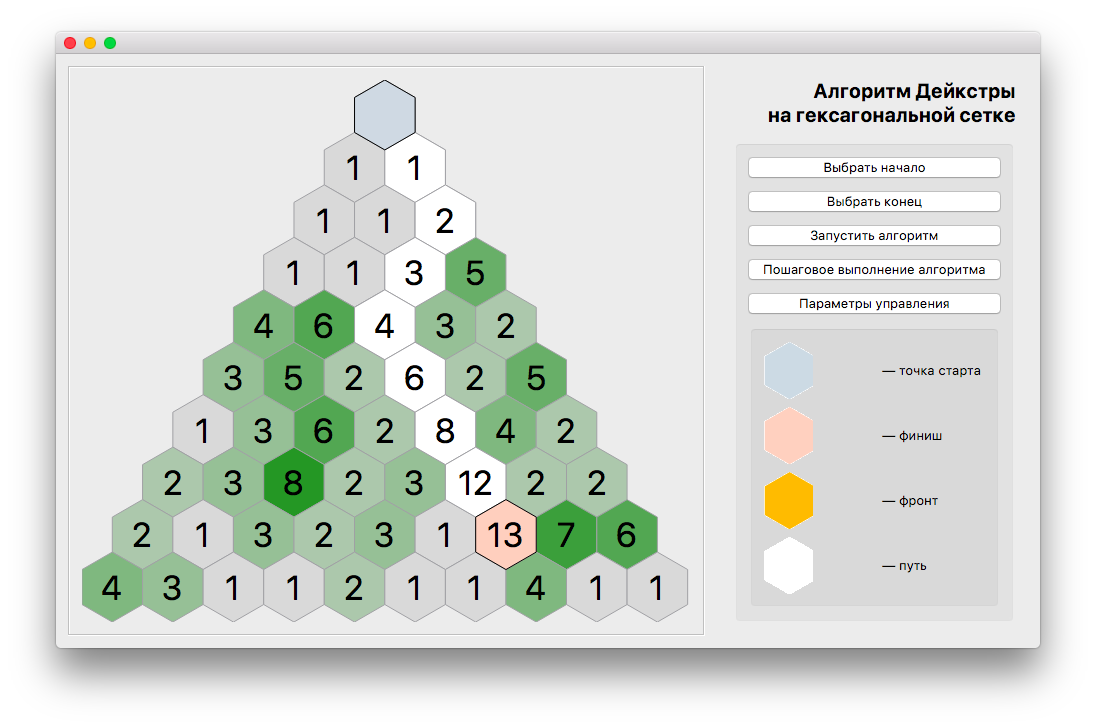
\includegraphics[width=1\linewidth]{inc/img/path}
\caption{Путь.} %% подпись к рисунку
\label{axis:cube} %% метка рисунка для ссылки на него
\end{minipage}
\hfill 
\begin{minipage}[h]{0.47\linewidth}
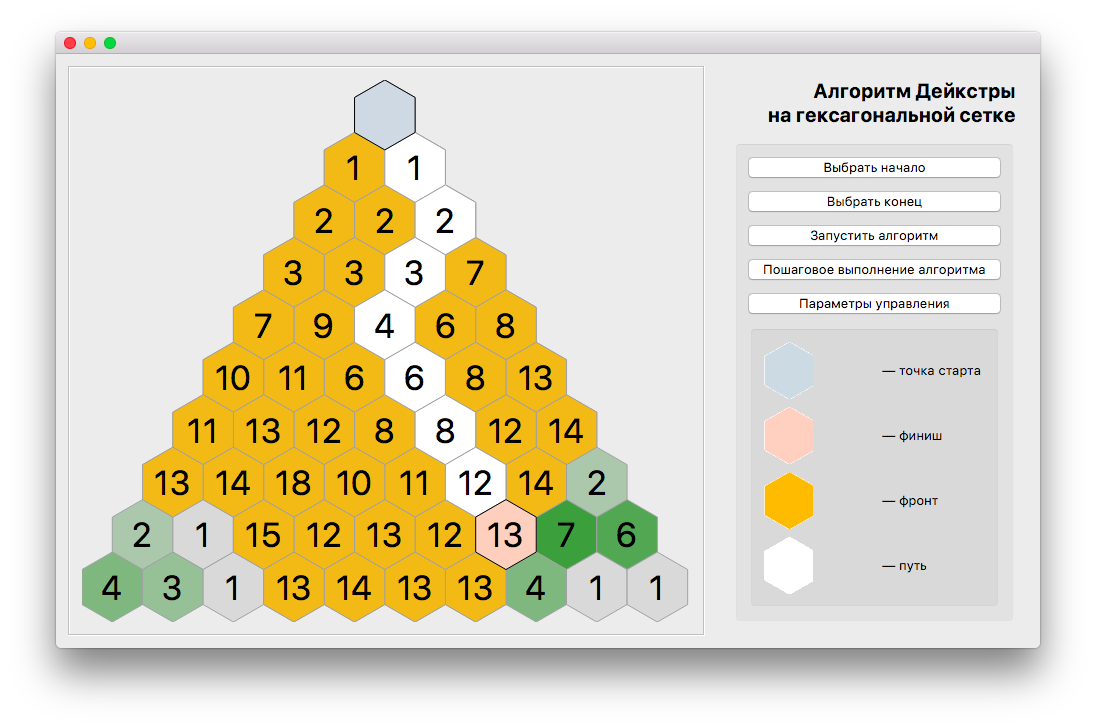
\includegraphics[width=1\linewidth]{inc/img/pathInAlg}
\caption{Путь с итерациями алгоритма.}
\label{axis:axial}
\end{minipage}
\end{center}
\end{figure}

%\chapter{Тестирование}
\label{cha:ch_5}
Процесс тестирования необходимо разделить на этапы:
\begin{enumerate}
	\item Низкая нагрузка --- размерность РТДРП в 10-20 элементов;
	\item Стандартная нагрузка --- РТДРП размерностью 30-60;
	\item Максимальная нагрузка --- РТДРП размерностью от 80 до 100.
\end{enumerate}

Раздел тестирования построен следующим образом:
\begin{enumerate}
	\item Указываются входные параметры (размерность РТДРП);
	\item Путь к директории, где расположены svg-файлы (/Tests/$\textbf{размерность РТДРП}$/svg);
	\item Количество svg-файлов в директории;
	\item Время отрисовки всех svg-файлов;
	\item Время выполнения алгоритма Дейкстры.
\end{enumerate}

\begin{table}[]
\centering
\label{my-label}
\begin{tabular}{|l|l|l|l|}
\hline
\textbf{Размерность} & \multicolumn{1}{|p{3cm}|}{\textbf{Кол-во svg-файлов}} & \multicolumn{1}{|p{3cm}|}{\textbf{Время отрисовки (мс)}} & \multicolumn{1}{|p{3cm}|}{\textbf{Время выполнения алгоритма Дейкстры (мс)}} \\ \hline
21                   & 6                          & 117.321                       & 13.011                                            \\ \hline
10                   & 4                          & 47.4077                       & 9.29                                              \\ \hline
50                   & 7                          & 549.783                       & 52.0214                                           \\ \hline
40                   & 8                          & 431.758                       & 73.3365                                           \\ \hline
60                   & 9                          & 1626.04                       & 312.842                                           \\ \hline
100                  & 11                         & 8389.83                       & 5161.01                                           \\ \hline
\end{tabular}
\caption{Результаты тестирования}
\end{table}

\backmatter %% Здесь заканчивается нумерованная часть документа и начинаются ссылки и
            %% заключение

%\Conclusion % заключение к отчёту

Текст заключения


\nocite{*}
\bibliographystyle{gost780u}
\bibliography{0-main}


%\appendix   % Тут идут приложения

%\chapter{Первое Приложение}

\end{document}
